\section{Monitor electricity consumption}
% Othe purpose, the fact that they have the 'same' client [although I think they are different research groups], and the differences,
% such as the data collection and the target user of the dashboards or project age etc.

\subsection{Initial Hypothesis}
\paragraph{Client} 
\ac{GEP} is a joint project of the \ac{VUB} (Free University of Brussels) and the \ac{UZB} (University Hospital of Brussels), both dutch and English-speaking research university located in Brussels, Belgium,
 with the motto: \textit{"Conquering darkness by science"} 
which purpose is to develop and operate a research campus in the Research park of Zellik with a focus on the following three research domains:
\begin{itemize}
    \item Energy and mobility transition
    \item Hospital of the future, part of \ac{BHC}
    \item Smart regions
\end{itemize}
With this research campus, Green Energy Park aims to bridge the gap between research, innovation, realization and exploitation, by acting as a large-scale living lab, expertise and training centre~\cite{Misc:vub_2020_green}.

\paragraph{Context Introduction}
\todo{Photo of \ac{BHC}}
As part of this project the \ac{BHC}, containing the academic Hospital, is a well-advanced
energy island owning and running a state-of-the-art microgrid that can work in island mode for
5 consecutive days. It includes a thermal and electricity grid, wastewater recovery, a high-
speed glass-fibre telecom network and a total of 33 \ac{HV} transformers divided over 18 \ac{HV} substations. 
Energy production and storage includes solar PV, CHP, 3 emergency generators,
and a total capacity of 2,5 MWh in battery storage, mainly under the form of UPS.
The microgrid serves the hospital complex, 250 student dwellings, the faculty of health
sciences, a primary school and a fitness centre. The microgrid system is conceived to go in
island mode with complete automatic transition in maximum 15 seconds in case of critical need
and in 3 min to comfort need. Cutting edge control
technology and maximal reliability are the focus points of this demonstration site.

\subsection{Goal(s), purpose \& critical factors}
\paragraph{Long term}
\begin{itemize}
    \item[$\circledcirc$] Grow Zensor into the main data hub for the Green Energy Park.
    \item[$\circledcirc$] Minimizing the energy losses and overall consumption, leading to a more profitable operation.
    \item[$\circledcirc$] Identify where the exact sources of this cost are and where the best opportunities for improvement lie.
\end{itemize}
\paragraph{Short term}
\begin{itemize}
    \item[$\circledcirc$] Having a view on the data, centralized and well accessible for multiple people in a structured way.
    \item[$\circledcirc$] Monitoring and tracking energy consumption in a production site resulting in more than mere energy bill reductions.
    \item[$\circledcirc$] Improve sustainability reducing energy need and peek request. 
\end{itemize}

\subsection{Project description by phases}
\begin{figure}[ht]
    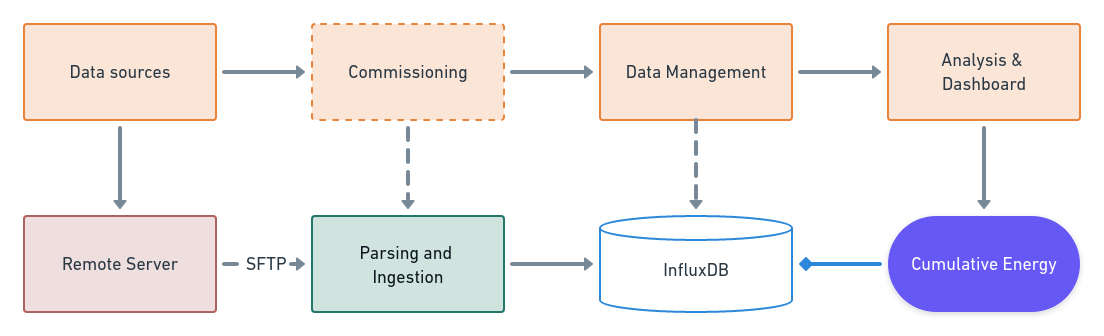
\includegraphics[width=\textwidth]{vub/analysis/4_phases.png}
    \caption{\ac{VUB}'s (light) project core stages}
    \label{fig:vub_stages}
\end{figure}
(Synopsis)
In this specific project the energy (related parameters) metered at the VUB BHC (the academic hospital in Jette) will have to be stored in our database and visualized for the client. 
They want to see some basic visualizations on it. This would need to happen 'fast'.
It's a limited dataset, no live link or permanent ingestion will have to be set up.
All the 'items' at that point should also have a link to the manual, spec-sheet... of the component (link to Snipe-It or other database).
The lay-out is a sort of 'ring' network with different 'nodes': the main transformers. These all have a code (C1, C3...). 
These have 'sub' transformers connected to them and on those transformers the 'consumers' are connected (or power sources). Sometimes a huge machine, sometimes an individual room.
The data would be 15-minute data over several years
In a first instance the dashboards need to have the same structure as the folders the .csv files are in. So: each folder containing .csv files should be a page in Grafana 
displaying the graphs of the series inn the .csv's in that folder.
In a second instance they want the entry point to be a map of the campus with the main transformers indicated and with a clickable link on each item such that the data can be consulted. 

\paragraph{Datasources}
\begin{figure}[ht]
    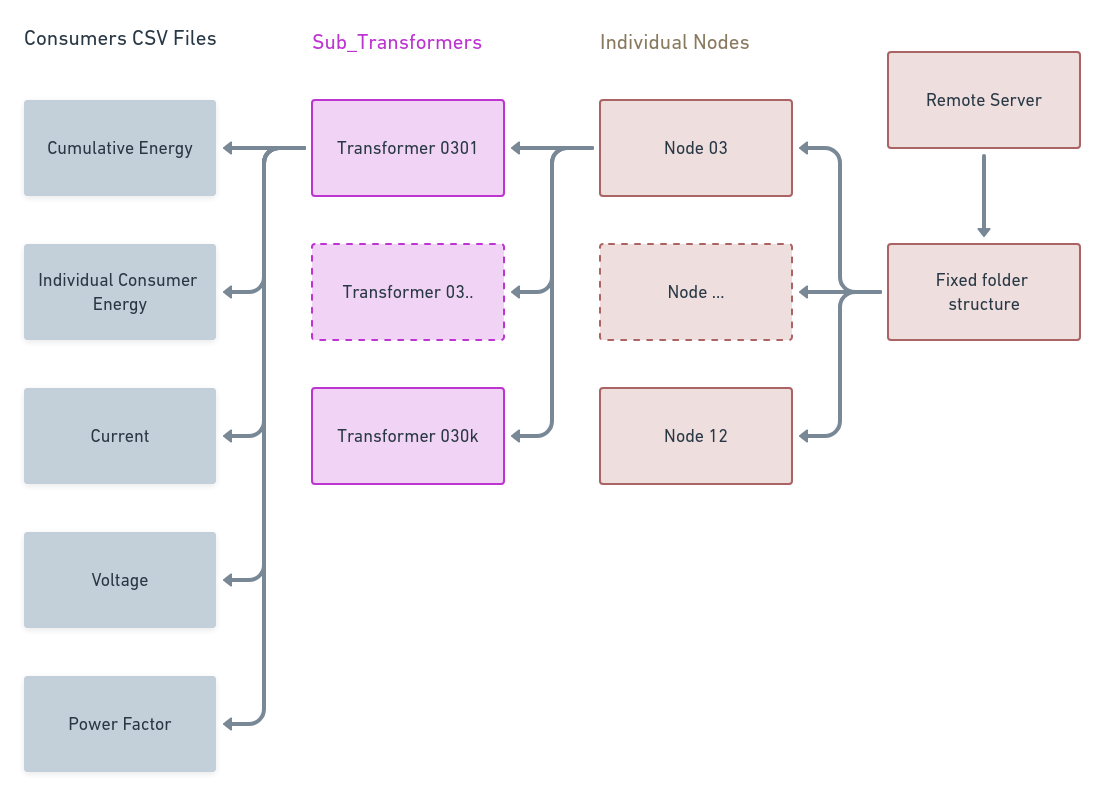
\includegraphics[width=\textwidth]{vub/analysis/folder_tree.png}
    \caption{\ac{VUB}'s remote server folder tree structure}
    \label{fig:vub_folder_tree}
\end{figure}

\paragraph{Commissioning}

\paragraph{Data Management}

\paragraph{Analysis}
\begin{figure}[ht]
    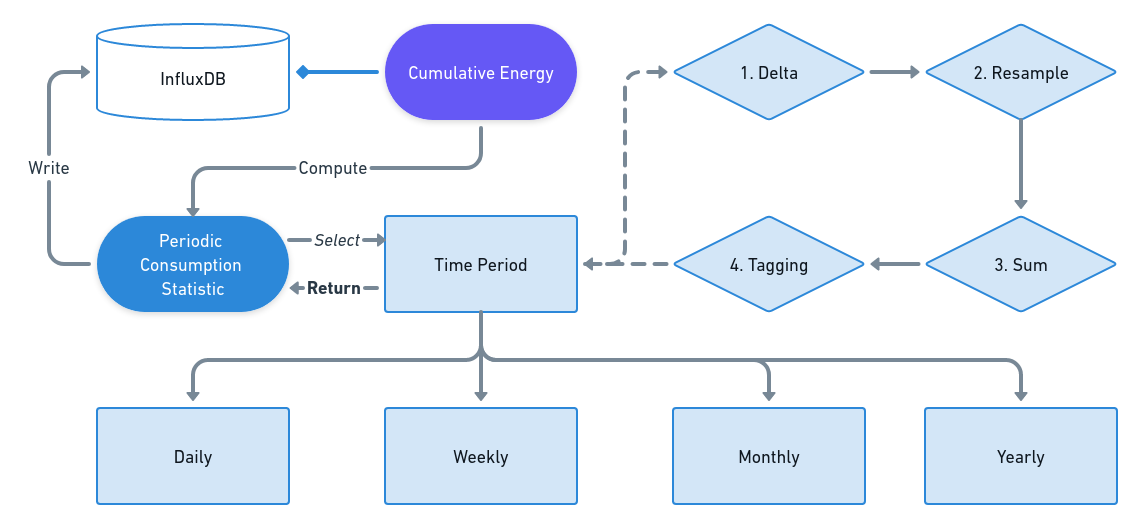
\includegraphics[width=\textwidth]{vub/analysis/analystic_flowchart.png}
    \caption{\ac{VUB}'s analytics chart}
    \label{fig:vub_anal_chart}
\end{figure}


\subsection{Conclusion}
